For the Electronics Lab course, the multimeter model that is being used is the 34405A. This multimeter helps measure features such as either true RMS AC or DC voltage and as well as true RMS AC or DC current. The range of the voltage on the multimeter goes from 10mV to 1000V, while the range for the current goes from 10mA to 10A \cite{34405A:3}. The input impedance of the multimeter is around 1M\si{\ohm} +/- 2\% for AC voltage while the input resistance for DC voltage is listed around 10M\si{\ohm} +/-2\%\cite{34405A:6}. The circuit in this lab is a simple series circuit, therefore the voltmeter acts as a voltage divider.\\
\\

\begin{figure}[h!]
\centering
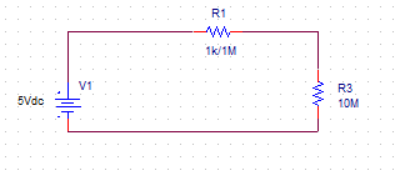
\includegraphics{voltmeterfinal.PNG}
\caption{Voltmeter Circuit Model}
\label{fig:Voltmeter_Pic}
\end{figure}

\begin{equation}
	\label{eq:vdvm}
	V_{DVM} = V_{Source}(\frac{R_{DVM}}{R_{DVM} + R}) 
\end{equation}

For the circuit with the voltmeter, students will measure the voltage across a voltmeter on a circuit using resistors of value 1kΩ and 1MΩ simultaneously. After measuring the voltage, equation \ref{eq:vdvm} can be used to find the impedance of the DVM from the voltmeter's voltage, the source's voltage, and the resistance R. To finish off this part of the experiment, the measured voltmeter impedance is compared to the manufacturer's results. 
